\documentclass{contest-set}
\usepackage{relsize}
\usepackage{tikz}
\usetikzlibrary{trees}
\usepackage{scalerel}
\usepackage{amsmath}
\usepackage{xcolor}
\usepackage{enumitem}

\title{$\scaleobj{1.5}{\pi}$-Day Contest}
\motto{``quantitas in quam cum multiflicetur diameter, proveniet circumferencia''}
\subheader{SLSS Computer Science Club}
\date{March 14, 2019}
\institute{Stephen Lewis Secondary School}
\organization{Computer Science Club}

\usetikzlibrary{arrows,decorations.markings}
\usepackage{caption}

\begin{document}
\makeatletter
\begin{titlepage}
	\centering
	{\itshape\LARGE\@institute\par}
	\vspace{1cm}
	{\scshape\Large\@organization\par}
	\vfill
	{{
	$\scaleobj{20}{\pi}$}\par}
	\vspace{2ex}
	{\parbox{0.8\linewidth}{\centering\scriptsize\itshape \textcolor{black!50}{3.141592653589793238462643383279502884197169399375105 
8209749445923078164062862089986280348253421170679...}} \par}
	\vspace{1.5cm}
    {\huge\bfseries \@title\par}
    \vspace{2ex}
% Bottom of the page
	{\large \@date\par}
	\vfill
\end{titlepage}
\makeatother

\maketitle
% RULES
\vspace{3ex}
\begin{enumerate}[listparindent=\parindent, labelwidth=!, labelindent=0pt]
    \item You have one (1) hour to complete this competition.
    \item You should assume that 
    \begin{itemize}
        \item all input is from the keyboard
        \item all output is to the screen
    \end{itemize}
    Be sure your output matches the expected output in terms of order, spacing, etc. \textit{IT MUST
    MATCH EXACTLY!}
    \item Do your own work; cheating will be dealt with harshly.
    \item Books and written materials are allowed. Internet resources of any kind are \textit{not} allowed. However, ``standard libraries'' for your programming languages are allowed (e.g. \texttt{STL} for \texttt{C++}, \texttt{System.*} for \texttt{C\#}, etc...).
    \item Your program will be run against test cases other than the provided sample cases.  Make sure to test your solution using other test cases. In addition, inefficient solutions may lose mark on some problems.
    \item You are allowed to submit your solution any number of times. No penalty will be applied for submission.
\end{enumerate}

\clearpage
\section{Race Around the Pie!}
Giovanni's dad is a baker, and is planning to bake an enormous lemon pie to celebrate. 

Giovanni and his friend Aurora will do a relay race around a quarter slice of the pie. Aurora will be running the outer curve of the slice, and she can do it running at a speed of $5$ metres per second. Giovanni will run both of the straight lines, and since he has to do a $90$ degree turn he is only able maintain an average speed of $4.5$ metres per second. The following figure represents their path:
\begin{figure}[h]
    \centering
    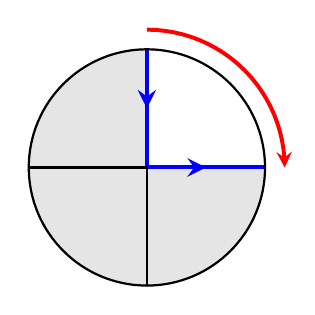
\begin{tikzpicture}[scale=0.5]
        \begin{scope}
            \clip (0,0) circle (3);
            \fill[black!10] (-3, 0) rectangle (0,3);
            \fill[black!10] (-3,-3) rectangle (3,0);
            % \fill[green] (0,0) rectangle (3,-3);
            \begin{scope}[very thick,decoration={
                markings,
                mark=at position 0.5 with {\arrow[>=stealth,scale=1.2]{>}}}]
                \draw [postaction={decorate},blue,thick,line width=0.5mm] (0,3) -- (0,0);
                \draw[postaction={decorate},blue,thick,line width=0.5mm] (0,0) -- (3,0);
            \end{scope}
            \draw [thick] (0,0) -- (0,-3);
            \draw [thick] (-3,0) -- (0,0);
            % \draw [] (-3,0) -- (3,0);
        \end{scope}
        \draw [thick] (0,0) circle (3);
        \draw [<-,>=stealth,red,thick,domain=0:90, line width=0.5mm] plot ({3.5*cos(\x)}, {3.5*sin(\x)});
        % \draw [->,>=stealth,blue,thick,line width=0.5mm] (0.3,2.7) -- (0.3,0.3);
    \end{tikzpicture}
    % \captionsetup{labelformat=empty}
    % \caption{The paths that Aurora an Giovanni will run on the lemon pie. The red represents Aurora's path and the blue represents Giovanni's path.}
\end{figure}

During the switch between runners, they will lose $0.5$ seconds. Assume they are both able to exactly follow the edge of the slice. 

Given a radius of $r$ metres for the quarter slice of lemon pie, output the total seconds it takes for Giovanni and Aurora to run one complete round around the perimeter.

\notewarning{For consistency in calculations, use $3.14$ in place of $\pi$.}

\inputformat
The input consists of a single-line containing a single floating-point number $r$ representing the radius of the lemon pie.

\constraints
$r \in \mathbb{R} \mid 1 \leq r \leq 10^6$

\outputformat
The output consists of a single floating-point number denoting the total time it takes for Giovanni and Aurora to run one complete round around the perimeter. Round to two decimal places.

\pushnewpage
\addsample{1}{1.26}
\addsample{5.93}{5.00}
\addsample{100}{76.34}

\clearpage
\section{Approximation}
We can approximate the value of $\pi$ by computing a partial summation that tends towards infinity. This type of summation is referred to as an \textit{infinite series}. A series is \textit{convergent} if the sequence of its partial sums tends to a limit; that is, they approach a finite value. Otherwise, the series is \textit{divergent}.

Using the following infinite series, approximate the value of $\pi$ using $n$ iterations to the $m$-th decimal place:
\begin{equation*}
    \pi \approx \frac{1}{2}\sum^\infty_{k=0}\frac{(k!)^2}{2(k+1)!}
\end{equation*}
An iteration refers to a single execution of the summation. Thus, computing $n$ iterations of the approximation refers to computing the summation where $0 \leq k < n$.

\inputformat
The input consists of single line containing two space separate integers $n$ and $m$ denoting the number of iterations of approximation and the number of decimal places to round to respectively.

\constraints
$1 \leq n \leq 10^4$\\
$1 \leq m \leq 10^3$

\outputformat
The approximated value of $\pi$ rounded to $m$ decimal places.

\addsample{19}{3.1415926535873004}

\newpage
\section{$\mathlarger{\mathlarger{\mathlarger{\pi}}}$-Tree}
There exists a very special type of tree called a $\pi$-tree. A tree is a $\pi$-tree \textit{if and only if} for every path from the root node to a leaf node, the sum of the nodes along the path is equal to $\pi$. Since $\pi$ is an irrational number and IEEE floats also come with some inaccuracies, we define $\alpha$ as being equal to $\pi$ if $3.139 \leq \alpha \leq 3.141$. Mathematically, a $\pi$-tree must satisfy the expression
\begin{equation*}
    \forall x \in \mathcal{P}, \sum^{|x|-1}_{i=0} x_i=\alpha,
\end{equation*}
where $\mathcal{P}$ represents a set containing all paths from the root node to an arbitrary leaf node.
For example, consider the following tree:
\begin{figure}[h]
    \centering
    \begin{tikzpicture}[level distance=1.5cm,
          level 1/.style={sibling distance=6cm},
          level 2/.style={sibling distance=3cm}]
          \node {$v_0=1$}
            child {node {$v_1=1$}
              child {node {$v_3=1.14$}}
              child {node {$v_4=1.14$}}
            }
            child {node {$v_2=0.14$}
            child {node {$v_5=1.5$}}
              child {node {$v_6=0.5$}
              child {node {$v_7=1.5$}}}
            };
        \end{tikzpicture}
\end{figure}

We can make it a $\pi$-tree by adding a new child node with the value of $0.5$ to node $v_5$. This way, all paths from the root to a leaf node have a sum which is equal to $\alpha$.

Given a tree with $n$ nodes and values $v_0$,$\ldots$,$v_{n-1}$, determine the minimum number of nodes that need to be added to make it into a $\pi$-tree. You are only allowed to add new nodes as children of leaf nodes.

\inputformat
The first line of input consists of a single integer $n$ which describes the number of nodes in the tree. The next $n$ lines of input contain a floating-point number which denotes the value of the $i$-th node $v_i$. The final $n-1$ lines represent the node connections; each line contains two space-separated integers $i$ and $j$ that denote that $j$ is a child of $i$.

\pushnewpage

\constraints
$1 \leq n \leq 10^6$\\
$0 \leq i < n$\\
$0 \leq j < n$\\
$v_i \in \mathbb{R}$

\outputformat
The output consists of a single integer which describes the minimum number of nodes that need to be added to make the tree into a $\pi$-tree.

% \pushnewpage

% \addsampleExplanation
% {
% 3\\
% 1\\
% 2.14\\
% 2.14\\
% 0 1\\
% 0 2
% }
% {
% 0
% }
% {
% No nodes need to be added because the sum of all the nodes in each possible path is equal to $3.14$. The tree is already a $\pi$-tree.
% }

\addsampleExplanation
{
4\\
0.14\\
1\\
2\\
0.5\\
0 1\\
1 2\\
1 3
}
{
1
}
{
We need to add a child node to node $3$ with a value of $1.5$ in order to make the tree a $\pi$-tree.
}
\end{document}